\begin{pa} \label{PA:9.4} 

  The cross product of two vectors, $\vu$ and $\vv$, will itself be a
  {\em vector} denoted $\vu\times\vv$.  The direction of
  $\vu\times\vv$ is determined by the right-hand rule: if we point the
  index finger of our right hand in the direction of $\vu$ and our
  middle finger in the direction of $\vv$, then our thumb points in
  the direction of $\vu\times\vv$.

  \ba

  \item We begin by defining the cross products using the vectors $\vi$,
  $\vj$, and $\vk$.  Referring to Figure \ref{F:9.4.basis}, explain
  why $\vi$, $\vj$, $\vk$ in that order form a right-hand system. We then define $\vi \times \vj$ to be $\vk$ -- that is $\vi\times\vj = \vk$.  
  \item Now explain why $\vi$, $\vk$, and $-\vj$ in that order form a right-hand system. We then define $\vi \times \vk$ to be $-\vj$ -- that is  $\vi\times\vk=-\vj$.
  \item Continuing in this way, complete the missing entries in Table~\ref{T:9.4.cross.def}.
    \begin{table}[ht]
      \begin{center}
        \begin{tabular}{lll}
          $\vi\times\vj = \vk$ \hspace*{1in} &
          $\vi\times\vk = -\vj$ \hspace*{1in} &
          $\vj\times\vk = $\hspace*{1in} \\ \\
          $\vj\times\vi = $ &
          $\vk\times\vi = $ &
          $\vk\times\vj = $
        \end{tabular}
      \end{center}
      \caption{Table of cross products involving $\vi$, $\vj$, and $\vk$.} 
      \label{T:9.4.cross.def}
    \end{table}

  \item Up to this point, the products you have seen, such as the
    product of real numbers and the dot product of vectors, have been
    commutative, meaning that the product does not depend on the order
    of the terms.  For instance, $2\cdot5 = 5\cdot 2$.  The table
    above suggests, however, that the cross
    product is {\em anti-commutative}: for any vectors $\vu$ and $\vv$ in $\R^3$,  $\vu\times\vv =
    -\vv\times\vu$.  

    If we consider the case when $\vu=\vv$, this shows that
    $\vv\times\vv = -\vv\times\vv$.  What does this tell us about
    $\vv\times\vv$;  in particular, what vector is unchanged by
    scalar multiplication by $-1$?

  \item The cross product is also a {\em bilinear} operation, meaning
    that it interacts with scalar multiplication and vector addition
    as one would expect:  
    $(c\vu + \vv)\times\vw = c(\vu\times\vw) + \vv\times\vw$. For example, 
\[(2\vi + \vj) \times \vk = 2(\vi \times \vk) + (\vj \times \vk) = -2\vj + \vi.\]
Using this property along with Table~\ref{T:9.4.cross.def}, find the cross product $\vu\times\vv$ if
    $\vu = 2\vi + 3\vj$ and $\vv = -\vi + \vk$.

  \item Verify that the cross product $\vu\times\vv$ you just found in
    part (e) is
    orthogonal to both $\vu$ and $\vv$.

  \item Consider the vectors $\vu$ and $\vv$ in the $xy$-plane as
    shown below in Figure \ref{F:9.4.activity_1}.

    \begin{figure}[ht]
      \begin{center}
        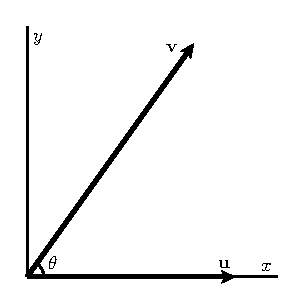
\includegraphics{figures/fig_9_4_activity_1.eps}
        \caption{Two vectors in the $xy$-plane}
        \label{F:9.4.activity_1}
      \end{center}
    \end{figure}

    Explain why $\vu = |\vu|\vi$ and $\vv = |\vv|\cos\theta \vi +
    |\vv|\sin\theta \vj$.  Then compute the length of $|\vu\times\vv|$.

  \item Multiplication of real numbers is {\em associative}, which
    means, for instance, that $(2\cdot 5)\cdot 3 = 2\cdot(5\cdot 3)$.
    Is it true that the cross product of vectors is associative?  For
    instance, is it true that
    $(\vi\times\vj)\times\vj = \vi\times(\vj\times\vj)$?

    \ea




\end{pa} 

\begin{activitySolution}
  \ba

  \item If we point the index finger of our right hand in the direction of $\vi$ and our middle finger in the direction of $\vj$, then our thumb points in the direction of $\vk$. So $\vi$, $\vj$, and $\vk$ form a right hand system.  
  \item If we point the index finger of our right hand in the direction of $\vi$ and our middle finger in the direction of $\vk$, then our thumb points in the opposite direction of $\vj$. So $\vi$, $\vk$, and $-\vj$ form a right hand system. 
  \item The cross products of combinations of the standard unit vectors are shown in the figure below. 
%   \begin{table}[ht]
     \begin{center}
       \begin{tabular}{lll}
          $\vi\times\vj = \vk$ \hspace*{1in} &
          $\vi\times\vk = -\vj$ \hspace*{1in} &
          $\vj\times\vk = \vi$\hspace*{1in} \\ \\
          $\vj\times\vi = -\vk$ &
          $\vk\times\vi = \vj$ &
          $\vk\times\vj = -\vi$
       \end{tabular}
      \end{center}
%      \caption{Table of cross products involving $\vi$, $\vj$, and $\vk$.} 
 %     \label{T:9.4.cross.def_sol}
 %  \end{table}

  \item The only vector that is unchanged by scalar multiplication by $-1$ is the zero vector. So we conclude that $\vv \times \vv = \vzero$. 

  \item Using the bilinearity of the cross product we find that 
  \begin{align*}
\vu \times \vv &= (2\vi + 3\vj) \times (-\vi + \vk) \\
	&= -2(\vi \times \vi) + 2(\vi \times \vk) - 3 (\vj \times \vi) + 3(\vj \times \vk) \\
	&= -2 \vzero - 2\vj +3 \vk + 3\vi \\
	&= 3 \vi - 2 \vj + 3 \vk.
\end{align*}

  \item Recall that two nonzero vectors are orthogonal if their dot product is 0. Since 
\[\vu \cdot (\vu \times vv) = (2 \vi + 3 \vj) \cdot (3 \vi - 2 \vj + 3 \vk) = 6 - 6 = 0\]
and
\[\vv \cdot (\vu \times vv) = (- \vi +  \vk) \cdot (3 \vi - 2 \vj + 3 \vk) = -3 + 3 = 0,\]
it follows that $\vu \times \vv$ is orthogonal to both $\vu$ and $\vv$. 

  \item Since $\vu$ is parallel to $\vi$, it must be the case that $\vu$ is a scalar multiple of $\vi$. Now $\vi$ is a unit vector and the magnitude of $\vu$ is $|\vu|$, so $\vu = |\vu| \vi$. The vector $\vv$ forms the hypotenuse of a right triangle with the $x$-axis as base. The horizontal leg of this triangle is the vector $|\vv| \cos(\theta) \vi$ and the vertical leg is the vector $|\vv|\sin(\theta) \vj$. Geometrically, we can see that vector legs sum to the vector hypotenuse, so $\vv = |\vv| \cos(\theta) \vi + |\vv| \sin(\theta) \vj$. Then
\begin{align*}
|\vu \times \vv| &= |(|\vu| \vi) \times (|\vv| \cos(\theta) \vi + |\vv| \sin(\theta) \vj) | \\
	&=  ||\vu| |\vv| \cos(\theta) (\vi \times \vi) + |\vu| |\vv| \sin(\theta) (\vi \times \vj) | \\
	&= ||\vu| |\vv| \sin(\theta) \vk | \\
	&= |\vu| |\vv| |\sin(\theta) |. 
\end{align*}

  \item Note $(\vi\times\vj)\times\vj = \vk \times \vj = -\vi$ while $\vi\times(\vj\times\vj) = \vi \times \vzero = \vzero$. So the cross product is not an associative operation. 
    \ea

\end{activitySolution}

\afterpa 